\chapter{Declaration}

I, \thethesisauthor, hereby declare that:

\begin{itemize}

\item The work in this dissertation is my own work.

\item All sources used or referred to have been documented and
recognised.

\item This \MakeLowercase{\thethesistype} has not previously been
submitted in full or partial fulfilment of the requirements for
an equivalent or higher qualification at any other recognised
educational institute.

\end{itemize}

%% You could of course include your signature electronically if you want to be fancy
%% Scanning and convert to eps should do the trick
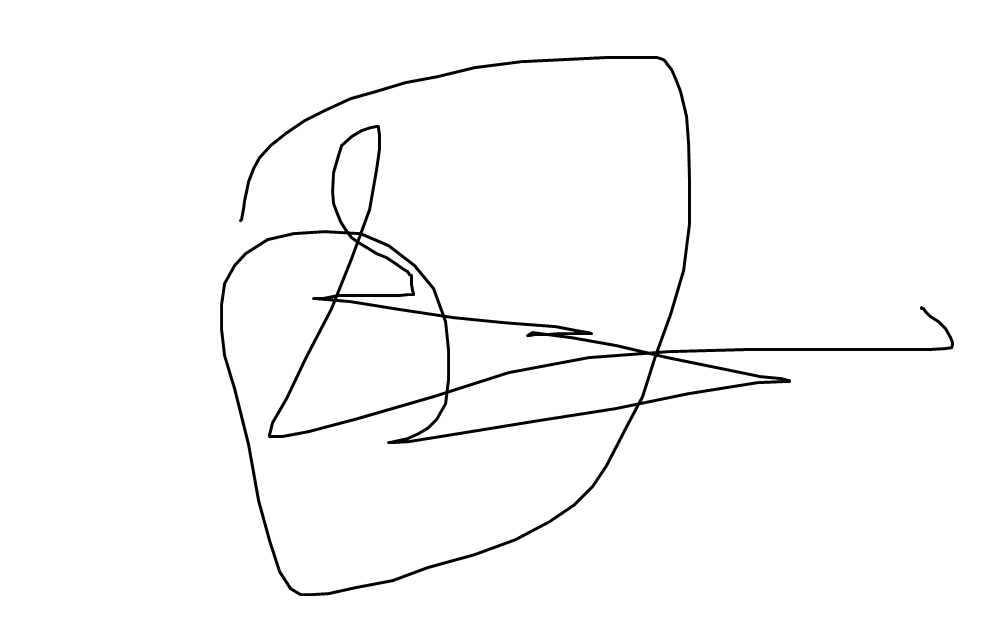
\includegraphics[width=40mm]{./figures/signature}
%% or you could just leave some space for it
\rule[0mm]{0mm}{40mm}

\rule[0mm]{70mm}{0.3mm}

\thethesisauthor

%\chapter*{Dedication}
%This thesis is dedicated to the memory of my father, \textbf{Anton van Heerden}.
%\textit{My father game me the greatest gift anyone could give another person...he believed in me.}

%Till we meet again dad.

\chapter{Acknowledgements}

Foremost, I would like to express my sincere gratitude to my supervisors Prof. Reinhardt A. Botha and Prof. Bertram P. Haskins for their continuous support during my Master's study. Furthermore, I would like to express my gratitude for their patience, motivation, enthusiasm, and immense knowledge. Their guidance assisted me throughout the research and writing of this dissertation. I could not have imagined having better supervisors for my Master's study.

Furthermore, I would like to thank the following benefactors for their financial assistance:

\begin{itemize}
	\item The financial assistance of the National Research Foundation (NRF) towards this research is hereby acknowledged. Opinions expressed and conclusions arrived at, are those of the authors, and are not necessarily to be attributed to the National Research Foundation.
	\item The financial assistance of the Nelson Mandela University's Post Graduate Research Scholarship (PGRS) is also hereby acknowledged.
\end{itemize}

Finally, I must express my very profound gratitude to my parents for providing me with unfailing support and continuous encouragement throughout the process of researching and writing this dissertation. This accomplishment would not have been possible without you. Thank you.

\chapter{Abstract}
The amount of information generated lately leads to information overload and impacted researchers’ decision-making capabilities. Researchers have access to a variety of digital libraries to retrieve information. Digital libraries often offer access to a number of journal articles and books. Although digital libraries have search mechanisms it still takes lots of time to find related research papers.

The main aim of this study was to develop a model that use Machine Learning techniques to recommend related research papers. The conceptual model was informed by literature on recommender systems in other domains. Furthermore, a literature survey on machine learning techniques helped identify candidate techniques that could be used.

The model comprises of four phases. These phases are completed twice, the first time for learning from the data and the second time when a recommendation is seeked. The four phases are: (1) identify and remove stopwords, (2) stemming the data, (3) identify the topics for the model and, (4) measuring similarity between documents.
 
The model is implemented and evaluated using a prototype to recommend research papers using a Natural Language Processing approach. The prototype undergone three iterations. The first iteration focused on understanding the problem domain by exploring how recommender systems and related techniques worked. The second iteration focused on pre-processing techniques, topic modeling and similarity measures of two probability distributions. The third iteration focused on refining the prototype, and documenting the lessons learned throughout the process. Practical lessons were learned while finalising the model and constructing the prototype. These practical lessons should help identify opportunities for future research.